\documentclass[10pt]{article}
\usepackage[a4paper,margin=20mm]{geometry}
\usepackage[T1]{fontenc}
\usepackage[utf8]{inputenc}
\usepackage{lmodern}
\usepackage{microtype}
\usepackage{amsmath,amssymb,amsthm,mathtools}
\usepackage{enumitem}
\usepackage{booktabs,tabularx,array,longtable}
\usepackage{xcolor}
\usepackage{hyperref}
\usepackage{tikz}
\usetikzlibrary{arrows.meta,positioning,shapes.geometric,fit,calc}
\hypersetup{colorlinks=true,linkcolor=black,citecolor=black,urlcolor=blue}
\setlist{nosep,leftmargin=*}
\setlength{\parskip}{3pt}
\setlength{\parindent}{1.25em}
\emergencystretch=2em
\newtheorem{definition}{Definition}[section]
\newtheorem{theorem}[definition]{Theorem}
\newtheorem{lemma}[definition]{Lemma}
\newtheorem{proposition}[definition]{Proposition}
\newtheorem{corollary}[definition]{Corollary}
\newtheorem{remark}[definition]{Remark}
\newtheorem{example}[definition]{Example}
\newtheorem{requirement}[definition]{Requirement}
\newcommand{\Res}{\operatorname{Res}}
\newcommand{\Ker}{\operatorname{Ker}}
\newcommand{\Choice}{\operatorname{Choice}}
\newcommand{\GCA}{\operatorname{GCA}}
\newcommand{\LCA}{\operatorname{LCA}}
\newcommand{\Adm}{\operatorname{Adm}}
\newcommand{\Succ}{\operatorname{Succ}}
\newcommand{\Loc}{\mathsf L}
\newcommand{\Glob}{\mathsf G}
\newcommand{\GC}{\mathsf{GC}}
\newcommand{\GI}{\mathsf{GI}}
\newcommand{\UB}{\mathsf{U}_B}
\newcommand{\NE}{\mathsf{NE}}
\newcommand{\TraceWF}{\mathsf{TraceWF}}
\newcommand{\TraceW}{\mathsf{TraceWarranted}}
\newcommand{\ValidReview}{\mathsf{ValidGCAReview}}
\newcommand{\Report}{\mathsf{Report}}
\newcommand{\CA}{\textsf{conditionally accepted}}
\newcommand{\GCS}{\textsf{global coherence assessed}}
\newcommand{\Genome}{\mathcal H}
\newcommand{\Config}{\Sigma}
\newcommand{\Operands}{\Omega}
\newcommand{\Contexts}{\Gamma}
\newcommand{\Fit}{\operatorname{Fit}}
\newcommand{\Best}{\operatorname{Best}}
\newcommand{\ProjFit}{\widehat F}
\newcommand{\OntFit}{F^{\mathrm{ont}}}
\newcommand{\RealFit}{F^{\mathrm{real}}}
\newcommand{\Candidates}{\mathsf{Candidates}}
\newcommand{\Project}{\mathsf{Project}}
\newcommand{\Validate}{\mathsf{Validate}}
\newcommand{\Execute}{\mathsf{Execute}}
\newcommand{\BudgetUpdate}{\mathsf{BudgetUpdate}}
\newcommand{\Target}{\Theta}
\newcommand{\Bridge}{\mathsf{Br}}
\newcommand{\Und}{\mathsf{undetermined}}
\newcommand{\GCsub}{\mathsf{GC}_{\mathrm{sub}}}
\newcommand{\GCpub}{\mathsf{GC}_{\mathrm{pub}}}
\newcommand{\MR}{\mathsf{MR}}
\newcommand{\Carrier}{\mathsf{Carrier}}
\newcommand{\TargetAdeq}{\mathsf{TargetAdeq}}
\newcommand{\RootDerives}{\mathsf{RootDerives}}
\newcommand{\SelfContained}{\mathsf{SelfContained}}
\newcommand{\Legible}{\mathsf{Legible}}
\newcommand{\ArtifactFaithful}{\mathsf{ArtifactFaithful}}
\newcommand{\ReviewClosed}{\mathsf{ReviewClosed}}
% Generated from GCAExecutionStatus_v23.json. Do not edit manually.
\newcommand{\ExpectedOverallGCA}{\ensuremath{\GCsub}}
\newcommand{\ActualOverallGCA}{\ensuremath{\NE}}
\newcommand{\ActualOverallGCAText}{not executed}


\title{Target-Relative Residue and Sound Choice-Gated Closure for Finite Assessment Systems}
\author{Andy E. Williams\\Caribbean Center for Collective Intelligence, St. John's, Antigua and Barbuda\\Nobeah Foundation, Nairobi, Kenya\\\texttt{info@cc4ci.org}}
\date{}

\begin{document}
\maketitle


\begin{abstract}
Let $X$ be a state space, $q:X\to Y$ an operative observation, and $\delta:X\to D$ a target verdict.  The target-relative residue
\[
  \Res_\delta(q)=\Ker(q)\setminus\Ker(\delta)
\]
contains exactly the pairs that the observation identifies while the target separates them.  We prove that the residue is empty exactly when the target factors uniquely through the image of the observation.  We identify the target-image observation as canonical in the refinement preorder, prove monotonicity under refinement, and show that every target-sufficient refinement must separate every residual pair.

We then use this invariant to define a finite Choice-gated assessment system.  A registered instance fixes a target, a target-adequate boundary, a policy-selected inclusion-minimal operand graph, native execution contexts and bridges, a finite candidate grammar, projected-fitness semantics, budgets, and record schemas.  Every local, global, and meta-level action is totally comparable by projected fitness for the same fixed target.  Every non-root recursive assessment is emitted by Choice after parent-mode information has been erased.  Progress totality and well-founded decrease yield a terminal bounded verdict.

The central result is a sound bounded-closure theorem: if native assessors and bridges are sound, candidate comparison is target-relative and complete for the registered grammar, parent-mode noninterference and progress hold, and a substantively warranted terminal trace derives global coherence, then every admissible completion consistent with the registered boundary has the root target verdict.  We also prove a target-selection theorem preventing a narrowed assessment target from standing in for a requested overall target, a finite relative-completeness theorem, strict separation examples for global-only and local-only recursion, and a projected-fitness margin theorem.

For journal use, the assessed object includes the article's mathematical core, carrier adequacy, artifact fidelity, recommendation-changing referee challenges, and submission-stage editorial status in one functional genome.  A detachable carrier recommendation of major revision is incompatible with an overall globally coherent submission-stage verdict.  Version 23 is written under the explicit design hypothesis that a fresh carrier-complete assessment returns $\GCsub$.  That hypothesis is not represented as an executed certificate: before the independent Claude Code audit, the recorded actual status is \ActualOverallGCA.  The package supplies a frozen carrier-complete review instance, schemas, a non-executable trace template, qpdf and Lean check scripts, and a structural output gate.  Claude Code must independently execute the review, produce node-specific Choice and execution records, import every recommendation-changing objection, and write a hash-bound external status record from the actual result without changing the frozen manuscript inputs.
\end{abstract}

\noindent\textbf{Keywords:} target-relative residue; factorization; assessment logic; Choice function; functional genome; global coherence; claim graph; proof certificates.




\section{Introduction}

This section states the representation, control, closure, and carrier problems addressed by the paper.  The representation problem is that an observation may be exact in its own codomain while erasing a distinction required by a declared target.  The control problem is that recursive assessment becomes self-sealing when the assessment mode of a parent is inherited by its successors rather than reselected by target-relative fitness.  The closure problem is that a trace can be structurally complete while lacking a semantic connection between its leaf warrants and its root verdict.  The carrier problem is that a mathematically coherent core can be transmitted through a manuscript that remains unsuitable for the target journal; excluding that carrier result from the root target creates a target-substitution error rather than a globally coherent submission.

Suppose an evaluator receives only $q(x)$ but must return $\delta(x)$.  If $q(x)=q(y)$ while $\delta(x)\neq\delta(y)$, no deterministic evaluator seeing only $q$ can be correct at both states.  The obstruction is target-relative loss of distinction.  The first theorem family isolates this loss as residue, characterizes its disappearance by factorization, identifies the canonical target-sufficient observation, and turns every residual pair into a necessary refinement obligation.

The same invariant applies to assessment targets.  Let $q_{\mathrm{frozen}}$ report the verdict produced by a frozen assessment target and let $\delta_{\mathrm{req}}$ report the verdict required by the user's overall target.  If two package states receive the same frozen-target verdict but different overall carrier verdicts, they form a target-selection residual pair.  A certificate produced from the frozen target cannot then certify the requested target.  This is the exact failure that occurs when model-internal coherence is certified while journal novelty, significance, transmission fitness, or artifact fidelity are moved into a detachable carrier verdict.

For recursive assessment, the required transition is
\[
  \text{execution}\longrightarrow\text{successor state}
  \longrightarrow\Choice\longrightarrow\text{next action},
\]
not $\Glob\to\Glob$ or $\Loc\to\Loc$.  Local assessment, global assessment, decomposition, information acquisition, model revision, rollback, and bounded halt are uniformly typed candidate paths.  Every available path has a projected fitness for the fixed target.  A multidimensional outcome record may expose adequacy, residue, preservation, warrant, viability, legibility, and cost, but the target-indexed policy must convert those effects into a total comparison before Choice occurs.

The paper's central theorem connects the residue semantics to terminal assessment.  A registered partial trace is interpreted as an observation of a space of admissible completions.  Root global coherence is sound only if all completions identified by the terminal trace receive the same root verdict and that verdict is the requested overall verdict.  This requires sound native assessors, target-preserving bridges, target-complete finite candidate generation, parent-mode noninterference, progress, trace coverage, substantive warrant, and sound root aggregation.  The theorem is conditional on these explicit interfaces; it does not define a predicate named ``sound'' and then infer soundness by unpacking the name.

The journal-facing assessed object is
\[
  P_J=(P_{\mathrm{formal}},P_{\mathrm{carrier}},P_{\mathrm{artifact}},
  P_{\mathrm{review}},P_{\mathrm{editorial\ stage}}).
\]
The carrier component contains scope fit, theorem centrality, novelty, significance, self-containment, legibility, related-work adequacy, length and format compliance, and the recommendation produced by a fresh review.  The artifact component contains source/PDF identity, structural PDF checks, rendered-page inspection, theorem-to-Lean correspondence, and the eventual Lean build certificate.  Recommendation-changing reviewer objections are imported as typed challenges.  The submission-stage target does not assert a future editorial acceptance event, but it requires the present carrier to warrant an accept recommendation or only non-root-changing production edits.  A live major-revision condition blocks $\GCsub$.

The formal contributions are:
\begin{enumerate}
  \item target-relative residue, image-relative factorization, evaluator obstruction, canonical target observation, refinement monotonicity, and universal residual-pair splitting;
  \item target-selection sufficiency: a frozen assessment target certifies the requested overall target exactly when the requested verdict factors through the frozen-target observation;
  \item a typed projected-fitness pipeline and total-preorder Choice function over local, global, and meta-actions;
  \item policy-selected inclusion-minimal operands from a finite target-complete family, with omitted target-relevant distinctions retained as residue;
  \item parent-mode-history erasure, information-flow noninterference, and strict successor-specific mode emission;
  \item progress plus well-founded termination and transition-conjugacy invariance;
  \item sound bounded Choice-gated closure over admissible completion spaces;
  \item relative completeness for the finite registered fragment under sufficient budget and fair execution;
  \item strict separation examples showing that both global-only and local-only recursion can fail where Choice-gated recursion succeeds;
  \item projected-to-ontic Choice stability under a strict fitness margin and bounded projection error;
  \item carrier-complete root aggregation, under which a recommendation of major revision cannot coexist with overall $\GCsub$; and
  \item an executable review contract that distinguishes a design hypothesis from an actual independently produced certificate.
\end{enumerate}

The global-coherence verdict set is $\{\GC,\GI,\UB\}$.  The separate status $\NE$ means that the registered assessment was not executed or failed its output gate.  Hence $\NE\neq\UB$: $\UB$ is available only after an actual bounded traversal leaves unresolved root-relevant residue.  The Version-23 manuscript is organized around the expected submission-stage verdict $\ExpectedOverallGCA$, but the package status remains $\ActualOverallGCA$ until Claude Code executes the frozen carrier-complete instance.  This prevents an anticipated result from becoming a premise or a falsely certified output.

The remainder of the article first develops the residue theorem family, then applies it to target adequacy, defines finite Choice and traversal, proves sound closure and separation, and finally specifies the carrier-complete article instance and independent execution protocol.

\section{Target-relative residue}

This section defines the central invariant and proves the representation results used by the assessment calculus.  The payoff is an exact criterion for when an observation contains enough information for a specified verdict and an exact description of what any successful refinement must add.

\begin{definition}[Target assessment frame]
A target assessment frame is a triple
\[
  \mathcal F_\delta=(X,D,\delta),
\]
where $X$ is a state space, $D$ is a verdict space, and $\delta:X\to D$ is total.  An operative observation is a total map
\[
  q:X\to\operatorname{im}(q).
\]
For a map $f$, its kernel relation is
\[
  \Ker(f)=\{(x,y)\in X^2:f(x)=f(y)\}.
\]
\end{definition}

\begin{definition}[Target-relative residue]
The target-relative residue of $q$ is
\[
  \Res_\delta(q)=\Ker(q)\setminus\Ker(\delta).
\]
A pair in $\Res_\delta(q)$ is a residual pair.  The observation is \emph{target sufficient} when $\Res_\delta(q)=\varnothing$.
\end{definition}

The definition is deliberately relative to a target.  The same observation can be sufficient for one verdict and insufficient for another.  This prevents a global assessment from being justified merely by the existence of information outside a local context: the omitted information must distinguish states that the fixed target distinguishes.

\begin{theorem}[Image-relative factorization]\label{thm:factorization}
For every observation $q:X\to\operatorname{im}(q)$, the following are equivalent.
\begin{enumerate}
  \item $\Res_\delta(q)=\varnothing$.
  \item $\delta$ is constant on every fibre of $q$.
  \item There is a unique map $\bar\delta:\operatorname{im}(q)\to D$ satisfying
  \[
    \delta=\bar\delta\circ q.
  \]
\end{enumerate}
\end{theorem}

\begin{proof}
The first two clauses both state $\Ker(q)\subseteq\Ker(\delta)$.  Under this inclusion define $\bar\delta(q(x))=\delta(x)$.  If $q(x)=q(y)$, fibre constancy gives $\delta(x)=\delta(y)$, so the definition is well defined.  Since $q$ is surjective onto its image, the factor map is unique.  Conversely, a factorization gives
\[
  q(x)=q(y)\Longrightarrow \bar\delta(q(x))=\bar\delta(q(y))
  \Longrightarrow\delta(x)=\delta(y),
\]
so the residue is empty.
\end{proof}

\begin{corollary}[Evaluator obstruction]\label{cor:evaluator}
If $(x,y)\in\Res_\delta(q)$, no deterministic evaluator depending only on $q$ is correct at both $x$ and $y$.
\end{corollary}

\begin{proof}
If $e$ were correct at both states, then
\[
  \delta(x)=e(q(x))=e(q(y))=\delta(y),
\]
contradicting the definition of a residual pair.
\end{proof}

\begin{proposition}[Refinement monotonicity]\label{prop:monotonicity}
If $q=h\circ q'$ for some map $h$, then
\[
  \Res_\delta(q')\subseteq\Res_\delta(q).
\]
\end{proposition}

\begin{proof}
The factorization $q=h\circ q'$ implies $\Ker(q')\subseteq\Ker(q)$.  Removing the same target kernel from both relations yields the inclusion.
\end{proof}

Thus a finer observation cannot introduce a residual pair that was absent from the coarser observation.  It may nevertheless preserve existing residue if it refines distinctions irrelevant to the target.

\subsection{Canonical target observation}

This subsection identifies the least information content sufficient for the target.  It gives a normal form against which candidate observations can be compared without choosing a particular representation language.

\begin{definition}[Target-image observation]
Define
\[
  q_\delta:X\to\operatorname{im}(\delta),\qquad
  q_\delta(x)=\delta(x).
\]
\end{definition}

\begin{definition}[Observation refinement preorder]
For observations $r:X\to R$ and $s:X\to S$, write $r\preceq s$ when $r=h\circ s$ for some map $h$; equivalently, $s$ is at least as discriminating as $r$.
\end{definition}

\begin{theorem}[Canonical least sufficient observation]\label{thm:canonical}
For every target-sufficient observation $s:X\to O$, let
\[
  \widehat s:X\to\operatorname{im}(s),\qquad
  \widehat s(x)=s(x)
\]
be its corestriction.  There is a unique map
\[
  \phi_s:\operatorname{im}(s)\to\operatorname{im}(\delta)
\]
such that
\[
  q_\delta=\phi_s\circ\widehat s.
\]
Hence $q_\delta\preceq\widehat s$ for every sufficient $s$.  Moreover, any sufficient observation $r$ satisfying $r\preceq s$ for every sufficient $s$ has the same kernel as $q_\delta$ and its image is uniquely isomorphic to $\operatorname{im}(\delta)$ over $X$.
\end{theorem}

\begin{proof}
Target sufficiency makes $\delta$ constant on fibres of $s$.  Define $\phi_s(\widehat s(x))=q_\delta(x)$.  This is well defined by fibre constancy and unique because $\widehat s$ is surjective onto $\operatorname{im}(s)$, proving $q_\delta\preceq\widehat s$.

Now suppose $r$ is sufficient and below every sufficient observation.  Since $q_\delta$ is sufficient, $r\preceq q_\delta$, so $\Ker(q_\delta)\subseteq\Ker(r)$.  Since $r$ is sufficient, the first part gives $q_\delta\preceq r$, so $\Ker(r)\subseteq\Ker(q_\delta)$.  The kernels are equal.  The maps induced between their images by the two factorizations are inverse because both corestrictions are surjective.  Thus the images are uniquely isomorphic over $X$.
\end{proof}

\begin{theorem}[Universal splitting obligation]\label{thm:splitting}
If $(x,y)\in\Res_\delta(q)$, then every target-sufficient observation $s$ satisfies $s(x)\neq s(y)$.
\end{theorem}

\begin{proof}
The residual pair gives $\delta(x)\neq\delta(y)$.  If $s(x)=s(y)$, target sufficiency would imply $\delta(x)=\delta(y)$, a contradiction.
\end{proof}

\begin{definition}[Refinement obligation]
A refinement obligation generated by a residual pair is the tuple
\[
  \omega=(x,y,q(x)=q(y),\delta(x)\neq\delta(y)).
\]
A successor observation discharges $\omega$ only by separating $x$ and $y$.
\end{definition}

Theorem~\ref{thm:splitting} is independent of the refinement mechanism.  A richer proof system, a broader literature search, an artifact reconstruction, or a cross-context bridge may all discharge the same obligation if they expose the missing target distinction.  The theorem does not guarantee termination of repeated refinement.  Termination requires a finite target quotient, a well-founded precision order, a decreasing unresolved-residue measure, or another explicit progress certificate.



\section{Target selection and carrier-complete scope}

This section applies the residue invariant to the assessment target itself.  The payoff is a formal prohibition on certifying a narrowed model-internal target as though it were the requested overall journal-submission target.

\begin{definition}[Requested and frozen verdict maps]
Let $X_J$ be the space of admissible package states at a fixed submission stage.  The requested overall verdict map is
\[
  \delta_J:X_J\to D_J,
\]
where $D_J$ records the overall submission-stage carrier verdict.  A frozen assessment target induces an observation
\[
  q_F:X_J\to O_F,
\]
which retains exactly the verdict information evaluated by that frozen target.
\end{definition}

\begin{definition}[Target-adequate frozen target]
The frozen target is adequate for the requested target when
\[
  \Res_{\delta_J}(q_F)=\varnothing.
\]
Equivalently, every two package states identified by the frozen target receive the same requested overall verdict.
\end{definition}

\begin{theorem}[Target-selection sufficiency]\label{thm:target-selection}
The frozen assessment target is sufficient for the requested overall carrier target if and only if there is a unique map
\[
  \psi:\operatorname{im}(q_F)\to D_J
\]
such that
\[
  \delta_J=\psi\circ \widehat q_F,
\]
where $\widehat q_F:X_J\to\operatorname{im}(q_F)$ is the corestriction.
Every pair $(x,y)$ satisfying $q_F(x)=q_F(y)$ but $\delta_J(x)\neq\delta_J(y)$ is a target-selection residual pair and blocks certification of the requested target from the frozen target.
\end{theorem}

\begin{proof}
Apply Theorem~\ref{thm:factorization} with state space $X_J$, observation $q_F$, and requested verdict $\delta_J$.  The final sentence is the evaluator obstruction specialized to assessment-target selection.
\end{proof}

\begin{example}[Detachable carrier verdict]
Let $x$ and $y$ have the same mathematical theorem package and therefore the same model-internal verdict.  Suppose $x$ states the central theorem accurately, proves novelty against the relevant baseline, includes faithful artifacts, and warrants an accept recommendation, while $y$ overstates the theorem, omits the novelty comparison, and warrants major revision.  A model-internal observation can identify $x$ and $y$, but the requested overall submission verdict separates them.  They are a target-selection residual pair.  The model-internal target is therefore insufficient for the requested carrier-complete target.
\end{example}

\begin{definition}[Carrier-complete submission object]
The submission-stage assessed object is
\[
  P_J=(F,C,A,R,E_s),
\]
where $F$ is the formal theorem package, $C$ the article carrier, $A$ the artifact package, $R$ the registered review history and open challenge state, and $E_s$ the submission-stage editorial state.  The target includes present scope fit, novelty, significance, theorem centrality, self-containment, legibility, artifact fidelity, and review-objection closure.  It does not assert a future journal decision.
\end{definition}

\begin{definition}[Stage-indexed targets]
The submission-stage target $\Target_J^{\mathrm{sub}}$ asks whether the present package is globally coherent as a submission and warrants acceptance or only non-root-changing production edits.  The publication-stage target $\Target_J^{\mathrm{pub}}$ additionally includes the actual editorial decision, completion of required revisions, and identity of the accepted artifacts.  An assessment may return $\GCsub$ before the journal acts; it may return $\GCpub$ only in a successor instance containing the authenticated acceptance event and final artifact hashes.
\end{definition}

\begin{requirement}[No target laundering]
Before any trace executes, a target-adequacy certificate must show that the frozen root target retains every distinction capable of changing the requested stage-indexed verdict.  A carrier coordinate may be omitted only with a typed irrelevance witness showing that every admissible variation is root invariant.
\end{requirement}

\begin{requirement}[No detachable major-revision result]
For the submission-stage root,
\[
  \MR\ \text{active and recommendation-changing}
  \quad\Longrightarrow\quad V_{\mathrm{overall}}\neq\GCsub.
\]
A repairable but unresolved major carrier defect yields conditional status or $\UB$; an incurable defeating defect yields $\GI$.
\end{requirement}


\section{Assessment operands and execution contexts}

This section defines the finite registered instance relative to which an assessment trace can be complete.  The same function family can be customized by selecting different operands and contexts, but the chosen review instance must be frozen before a verdict trace begins.

\begin{definition}[Claim package]
A claim package is $\mathcal P=(N,E,\lambda,\pi,\mathcal A)$, where $N$ is a finite set of registered nodes, $E$ a typed dependency relation, $\lambda$ assigns statements and node types, $\pi$ stores provenance and version history, and $\mathcal A$ is the set of declared artifacts.
\end{definition}

\begin{definition}[Assessment target]
An assessment target is
\[
  \Target=(X_\Target,D_\Target,\delta_\Target,\partial_\Target,
  T_\Target,U_\Target,H_\Target,J_\Target),
\]
where $\partial_\Target$ is the declared boundary, $H_\Target$ the recursive horizon, and $J_\Target$ the stage-indexed journal-carrier criterion when the assessed object is a submission.  The target is fixed before operands, contexts, candidates, modes, or expected verdicts are selected.  For Version 23, $J_\Target$ is the carrier-complete submission-stage target rather than a detachable model-internal target.
\end{definition}

\begin{definition}[Target-indexed comparison policy]
A comparison policy is
\[
  \Pi_\Target=(\rho_\Target,S_\Target,
  \preceq_\Target,\tau_\Target),
\]
where $\rho_\Target$ adjusts projected outcomes for registered uncertainty, $S_\Target$ maps adjusted outcomes into a fitness space $\mathbb F_\Target$, $\preceq_\Target$ is a total preorder, and $\tau_\Target$ selects only inside an equal greatest-fitness class.  The target and policy are fixed and hashed before candidate generation.
\end{definition}

\begin{definition}[Target-complete operand graph]
A finite rooted subgraph $G\subseteq\mathcal P$ is target complete when it is ancestor closed, dependency complete for its registered claim types, provenance preserving, and equipped with omission records such that every omitted object capable of changing the root verdict within $(\partial_\Target,H_\Target)$ is retained as unresolved residue.
\end{definition}

\begin{requirement}[Nonempty finite registered family]
The registered family $\mathfrak C_\Target$ is finite and nonempty.  The full finite claim graph with its omission records is registered as a fallback member, so target-complete selection is always defined.
\end{requirement}

\begin{definition}[Policy-selected inclusion-minimal operands]
The operand selector returns
\[
  \Operands_\Target^{\Pi}=\tau_\Omega
  \bigl(\operatorname{Min}_{\subseteq}\mathfrak C_\Target\bigr),
\]
where $\tau_\Omega$ is a deterministic policy-fixed selector over inclusion-minimal graphs.  The construction does not claim that a unique least graph exists unless a closure operator establishing one is separately proved.
\end{definition}

\begin{theorem}[Finite operand-selection existence]\label{thm:operand-selection}
Every nonempty finite registered family of target-complete operand graphs contains an inclusion-minimal member; therefore the policy-selected operand graph is defined.
\end{theorem}

\begin{proof}
Starting from any member, repeatedly replace it by a strict subgraph in the family whenever one exists.  Finiteness prevents an infinite descent, so the process reaches an inclusion-minimal member.  The fixed selector $\tau_\Omega$ then returns one member of the nonempty finite minimal set.
\end{proof}

This rule supplies a principled stopping condition.  The fact that an object could be elaborated, implemented, or formalized at another meta-level does not make it mandatory.  A request for expansion must identify a concrete admissible variation capable of changing the root target within the registered instance; otherwise the object remains conditionally accepted under its activation conditions.

\begin{definition}[Execution context]
For operand $o$, an execution context is
\[
  \kappa_o=(X_o,\Target_o,\partial_o,\mathcal R_o,
  \mathcal W_o,\mathcal D_o,q_o,B_o,H_o),
\]
containing the native state space, local target, boundary, rule, warrant, defeat, observation, budget, and history interfaces.
\end{definition}

\begin{definition}[Target bridge]
A bridge $\Bridge_o:D_o\to D_{\mathrm{parent}}$ is admissible only when a registered bridge-validation predicate warrants preservation of node identity, target meaning, boundary conditions, defeat reachability, and successor obligations.  A bridge whose validation remains conditional propagates that condition rather than silently converting it into unconditional parent warrant.
\end{definition}

\begin{definition}[Assessment configuration]
A configuration is
\[
\begin{aligned}
\Config=(
&\Operands,\Contexts,\Candidates,\Project,\rho_\Target,S_\Target,
\preceq_\Target,\tau_\Target,\\
&\Validate,\Execute,\Succ,\BudgetUpdate,\mathsf{Stop},B).
\end{aligned}
\]
Candidate generation is complete only relative to a fixed finite action grammar, context registry, and search horizon.
\end{definition}

\begin{definition}[Registered finite review instance]
A review instance is
\[
  \mathfrak R=(J,\mathcal P,\Target,\Pi_\Target,
  \partial_\Target,G_0,\mathcal G,H_\Target,
  \Config,B,\mathcal S,\mathcal J,\mathcal E),
\]
where $G_0$ is the policy-selected operand graph, $\mathcal G$ the finite candidate grammar, $\mathcal S$ the record-schema set, $\mathcal J$ the dated journal-profile snapshot, and $\mathcal E$ the carrier evidence registry.  All identity components are hashed.  Trace completeness is relative to $\mathfrak R$, never to the unbounded universe of describable objects.  The frozen instance also records the expected author-side outcome and the distinct actual execution status; the expected outcome has no role in Choice or root aggregation.
\end{definition}

\section{Candidate paths, projected fitness, and Choice}

This section corrects the control layer by distinguishing outcome projection from target-relative comparison.  Every available action is comparable by its fitness for the fixed target.  The choosing system ordinarily has access only to projected fitness, not to the action's unknown realized future contribution.

\subsection{Uniformly typed candidate paths}

\begin{definition}[Candidate action]
A candidate action is
\[
  a=(\mathsf{op},o,\kappa,\pi,\mathsf{cost},\mathsf{rollback}),
\]
where $\mathsf{op}$ is the invoked operator, $o$ the operand, $\kappa$ an admissible execution context, $\pi$ the projected transition interface, $\mathsf{cost}$ the budget effect, and $\mathsf{rollback}$ the recovery interface.  For a coherence-assessment operand, the finite candidate set can contain
\[
\begin{aligned}
  &\Loc_\kappa(o), &&\Glob_\gamma(o), &&\mathsf{Dec}_d(o),\\
  &\mathsf{Info}_i(o), &&\mathsf{Revise}_m(o),
  &&\mathsf{Rollback}_h(o),\quad\mathsf{Halt}_{\UB}(o).
\end{aligned}
\]
Every candidate has a projected fitness in the same target-relative fitness space.  The safe-halt action is always admissible, so the admissible candidate set is nonempty.  Completeness means completeness relative to the registered finite action grammar, context registry, and search horizon; it is not a claim that every conceptually possible action has been enumerated.
\end{definition}

\begin{definition}[Local assessment]
A local assessment $\LCA_o^\kappa$ evaluates $o$ using the native rules, warrants, defeats, and observation of one admissible context $\kappa$.  Its result is
\[
  r_o^{\Loc}=(v_o^{\Loc},W_o^{\Loc},R_o^{\Loc},C_o^{\Loc}),
\]
where $v$ is a native verdict, $W$ checked warrant, $R$ unresolved target-relative residue, and $C$ consumed cost.
\end{definition}

\begin{definition}[Global assessment]
A global assessment $\GCA_o^\gamma$ evaluates $o$ over a policy-selected inclusion-minimal target-complete family $\gamma$ of relevant contexts and checked bridges.  Its result is
\[
  r_o^{\Glob}=(v_o^{\Glob},W_o^{\Glob},R_o^{\Glob},C_o^{\Glob},T_o),
\]
where $T_o$ records the cross-context traversal.  Global assessment is not the union of all available information; it is a target-complete composition path competing with every other admissible path.
\end{definition}

Local and global describe support required for a particular target.  The image-relative factorization theorem is locally assessable in its mathematical proof context.  The claim that several theorem, control, traversal, and genome families compose into the article's root claim is globally assessable because the target depends on typed relations among those contexts.

\subsection{Ontic, projected, and realized fitness}

\begin{definition}[Projected-fitness pipeline]
For state $s$, candidate $a$, context $\kappa$, projection model $M$, and evidence $E$, the configured maps have types
\[
\begin{aligned}
\Project &: (s,a,\kappa,M,E)\longmapsto p_a\in\mathcal P_\Target,\\
\rho_\Target &: (p_a,E)\longmapsto \widetilde p_a\in\widetilde{\mathcal P}_\Target,\\
S_\Target &: \widetilde{\mathcal P}_\Target\longmapsto \mathbb F_\Target.
\end{aligned}
\]
The projected fitness is
\[
  \ProjFit_\Target(a\mid s,\kappa,M,E)
  =S_\Target\!\left(\rho_\Target(\Project(s,a,\kappa,M,E),E)\right).
\]
The ontic fitness $\OntFit_\Target(a\mid s,\kappa)$ is the action's actual contribution to the target, while $\RealFit_\Target(a,r)$ is registered after execution for calibration.
\end{definition}

A wrong projection can produce a wrong choice, but it does not make the actions intrinsically incomparable.  Uncertainty is included in the projected outcome and evaluated by the registered risk or uncertainty policy.  When the best way to improve target attainment is to obtain information or revise the model, Choice can emit that meta-action.

\begin{definition}[Projected outcome record]
For article assessment, the projection can expose
\[
  \mathbf z_\Target(a)=(A,Z,P,W,V,L,K),
\]
where $A$ is target adequacy, $Z$ unresolved target-relative residue, $P$ preservation of identity, boundary, and successor obligations, $W$ warrant and defeat reachability, $V$ viability and rollback, $L$ legibility, and $K$ cost.  A target-relative aggregator
\[
  S_\Target:\mathcal Z_\Target\to\mathbb F_\Target
\]
converts this record into a totally comparable fitness value.
\end{definition}

The aggregator can enforce hard noncompensation.  For example, failure of minimum adequacy, preservation, or viability can map an action to $\bot_\Target$ before remaining admissible records are compared lexicographically by
\[
  (A,-Z,P,W,V,L,-K).
\]
The coordinate priorities are fixed by the target policy.  A numerical score can represent the induced order on any finite candidate set without claiming that fitness is intrinsically cardinal.

\begin{definition}[Target-relative fitness preorder]
The fitness space $(\mathbb F_\Target,\preceq_\Target)$ is a total preorder: it is reflexive, transitive, and total.  Define
\[
  u\sim_\Target v
  \quad\Longleftrightarrow\quad
  u\preceq_\Target v\text{ and }v\preceq_\Target u.
\]
Thus any two actions are ordered or fitness-equivalent for the fixed target.
\end{definition}

Coordinate-wise dominance remains useful only as a pruning rule.  If the aggregator is monotone and one action is no worse in every target-effective feature and strictly better in one, the inferior action can be removed.  Failure of dominance does not establish fitness incomparability.

\begin{requirement}[Target and policy fixation]\label{req:same-target}
The target, uncertainty treatment, aggregator, total preorder, and tie rule are registered before candidate generation.  A target-hash or policy-hash change invalidates the Choice certificate.
\end{requirement}


\begin{requirement}[Registered candidate completeness]\label{req:candidate-complete}
For each state, $\Candidates$ must expose every action type in the finite registered grammar within the declared context registry and horizon.  A path that is presently inapplicable is retained explicitly with an inapplicability witness and bottom projected fitness rather than silently omitted.  Context-indexed variants may add candidates, but no grammar action type disappears.  A challenge alleging an omitted action must identify the grammar extension and explain how it can change the root target; otherwise it is an optional reconfiguration rather than a defect of the frozen instance.
\end{requirement}

\begin{requirement}[No target inflation]\label{req:no-inflation}
A desired mode or anticipated result may not enlarge the target, change success criteria, add dependencies, or omit alternatives merely to increase its projected fitness.
\end{requirement}

\subsection{The corrected Choice function}

\begin{definition}[Best-action set]
For state $s$ and its finite nonempty admissible set $\Adm(s,\Target)$, define
\[
\begin{aligned}
  \Best_\Target(s)=\{a\in\Adm(s,\Target):
  \ProjFit_\Target(b\mid s)
  \preceq_\Target
  \ProjFit_\Target(a\mid s)
  \text{ for every }b\in\Adm(s,\Target)\}.
\end{aligned}
\]
\end{definition}

\begin{definition}[FMI Choice]
The corrected Choice function is
\[
  \boxed{
  \Choice_\Target(s;\Config)
  =\tau_\Target\bigl(\Best_\Target(s)\bigr)}.
\]
The tie rule is fixed by the target policy and may select only from the equal greatest-fitness class.  It cannot reverse a strict fitness comparison.
\end{definition}

\begin{theorem}[Best-action existence]\label{thm:best-existence}
If the admissible candidate set is finite and nonempty and $\preceq_\Target$ is a total preorder, then $\Best_\Target(s)$ is nonempty.
\end{theorem}

\begin{proof}
Quotient the finite admissible set by $\sim_\Target$.  The quotient is a finite total order and therefore has a greatest equivalence class.  Its members are exactly $\Best_\Target(s)$.
\end{proof}

\begin{definition}[Choice-emission certificate]
A Choice-emission certificate stores the target and policy hashes, complete admissible candidate set, context and bridge of every candidate, projection model and evidence basis, projected outcome record and fitness value of every candidate, proof of total comparison, best-action class, tie rule and result, emitted action, budget effect, and typed defeat or recalibration conditions.
\end{definition}

\begin{theorem}[Local fitness emission]\label{thm:local-emission}
Let $a_\Loc=\Loc_{\kappa^*}(o)$ be admissible.  If
\[
  \ProjFit_\Target(a\mid s)
  \preceq_\Target
  \ProjFit_\Target(a_\Loc\mid s)
  \quad\text{for every admissible }a,
\]
and $\tau_\Target$ selects $a_\Loc$ from its best-action class, then
\[
  \Choice_\Target(s;\Config)=a_\Loc.
\]
If every other admissible action has strictly lower projected fitness, the conclusion is independent of the tie rule.
\end{theorem}

\begin{proof}
The comparison places $a_\Loc$ in $\Best_\Target(s)$.  The disclosed tie rule selects it.  Under strict superiority, the best-action class is the singleton $\{a_\Loc\}$.
\end{proof}

\begin{theorem}[Global fitness emission]\label{thm:global-emission}
Let $a_\Glob=\Glob_{\gamma^*}(o)$ be admissible.  If
\[
  \ProjFit_\Target(a\mid s)
  \preceq_\Target
  \ProjFit_\Target(a_\Glob\mid s)
  \quad\text{for every admissible }a,
\]
and $\tau_\Target$ selects $a_\Glob$ from its best-action class, then
\[
  \Choice_\Target(s;\Config)=a_\Glob.
\]
If every other admissible action has strictly lower projected fitness, the conclusion is independent of the tie rule.
\end{theorem}

\begin{proof}
Identical to Theorem~\ref{thm:local-emission}, with $a_\Glob$ in the equal greatest-fitness class.
\end{proof}

The substantive obligation is to establish the inequalities.  Empty local residue, native proof warrant, lower cost, and lower projection-error exposure can make local assessment strictly fitter.  A reachable local residual pair, a checked global path that discharges it, and preservation of hard conditions can make global assessment fitter.  Neither witness bypasses Choice: a global path may fail to resolve the residue or be inferior to decomposition, information acquisition, revision, rollback, or halting.

\begin{proposition}[Residue-based local preference]\label{prop:local-preference}
Assume the local observation is target sufficient, the local context supplies the required warrant and hard-condition preservation, and the fixed target aggregator assigns the local action a fitness value at least as great as every complete-set alternative.  Then the local action belongs to the best class; if the inequality is strict it is selected independently of the tie rule.  Residue and cost facts are evidential premises for the registered comparison, not substitutes for it.
\end{proposition}

\begin{proposition}[Residue-based global preference]\label{prop:global-preference}
Assume every local candidate retains a reachable target-relevant residual obligation, one global path discharges those obligations while preserving all hard conditions, and the fixed target aggregator assigns that global path a fitness value at least as great as every complete-set alternative.  Then it belongs to the best class; if the inequality is strict it is selected independently of the tie rule.
\end{proposition}

\begin{corollary}[No global-by-default rule]
The fact that the parent of $o$ was globally assessed is insufficient to derive global emission at $o$.
\end{corollary}

\begin{proof}
Parent mode is absent from the candidate projection and fitness comparison.  Global emission requires a successor-specific greatest-fitness certificate.
\end{proof}



\section{Choice-gated recursive traversal}

This section defines recursion, parent-mode noninterference, and terminal progress.  The relevant anti-inheritance result is an information-flow property: parent-mode information must not influence candidate generation, projection, fitness, or Choice indirectly through history.

\begin{definition}[Mode-history erasure]
Let $\mathsf{erase}_{\mathrm{pm}}:S\to\bar S$ remove the parent action's local/global tag and every history field from which that tag can be reconstructed, while preserving target-relevant evidence, provenance, budgets, and non-mode history.  The configured control maps are mode-history noninterfering when there exist maps on $\bar S$ such that
\[
\begin{aligned}
\Candidates&=\bar\Candidates\circ\mathsf{erase}_{\mathrm{pm}},\\
\Project&=\bar\Project\circ\mathsf{erase}_{\mathrm{pm}},\\
\ProjFit_\Target&=\bar F_\Target\circ\mathsf{erase}_{\mathrm{pm}},\\
\Choice_\Target&=\bar\Choice_\Target\circ\mathsf{erase}_{\mathrm{pm}}.
\end{aligned}
\]
\end{definition}

\begin{theorem}[Parent-mode noninterference]\label{thm:mode-independence}
If $\mathsf{erase}_{\mathrm{pm}}(s_1)=\mathsf{erase}_{\mathrm{pm}}(s_2)$, then the candidate sets, candidate-specific projections, projected fitness values, best classes, and Choice outputs at $s_1$ and $s_2$ are equal.
\end{theorem}

\begin{proof}
Each control map factors through the common erased state.  Equality of erased states therefore implies equality of the outputs of every factored map.
\end{proof}

\begin{definition}[Assessment execution record]
An execution record is
\[
  e=(s,h_\Target,h_\Pi,c,a,\kappa,\Validate(a),r,
  \RealFit_\Target(a,r),R,B_{\mathrm{before}},B_{\mathrm{after}},H'),
\]
where $c$ is the preceding Choice record.  An execution without a valid referenced Choice record is not a transition of the calculus.
\end{definition}

\begin{definition}[Choice-gated traversal]
For every non-root successor, the traversal performs
\[
  o\mapsto\Candidates(o)\mapsto\Project(o)
  \mapsto\Choice_\Target(o)\mapsto\Validate(a)
  \mapsto\Execute(a)\mapsto\Succ(e).
\]
A global execution may register successors but cannot directly invoke another global execution.
\end{definition}

\begin{theorem}[Successor-specific mode switching]\label{thm:mode-switch}
Assume mode-history noninterference.  If at a successor state an action whose mode differs from the parent mode has strictly greatest projected fitness in the complete registered candidate set, then Choice emits that action.  The conclusion is independent of the parent mode.
\end{theorem}

\begin{proof}
Noninterference makes the candidate set and projected-fitness comparison functions of the erased successor state.  Strict greatest fitness makes the best class a singleton, so the fixed tie rule emits the different-mode action.
\end{proof}

\begin{theorem}[No inherited global execution]\label{cor:no-inheritance}
Every non-root global execution has a preceding node-specific Choice certificate establishing that the emitted global path lies in the greatest projected-fitness class of the complete candidate set for the successor's fixed target.
\end{theorem}

\begin{proof}
Immediate from the Choice-gated traversal definition and the execution-record requirement.
\end{proof}

\begin{definition}[Progress and terminal totality]
Let $\mu:S\to W$ map states into a well-founded strict order.  A traversal is progress-total when every reachable state is either terminal with exactly one verdict in $\{\GC,\GI,\UB\}$ or has at least one validated executable successor, and every nonterminal transition strictly decreases $\mu$.
\end{definition}

\begin{theorem}[Progressive traversal termination]\label{thm:termination}
Every progress-total traversal terminates after finitely many transitions with exactly one verdict in $\{\GC,\GI,\UB\}$.
\end{theorem}

\begin{proof}
An infinite transition sequence would induce an infinite descending chain in $W$.  A finite sequence cannot end at a nonterminal deadlock because progress totality supplies a validated successor.  Hence it ends at a terminal verdict state.
\end{proof}

Positive real-valued costs without a lower bound do not establish termination.  The article instance uses natural-number budget components and a lexicographic structural measure.  Safe halt is included in the registered grammar and is required to be validated, executable, and verdict producing whenever no fitter progress action is available.

\begin{definition}[Execution budgets]
For trace $T$, $B_{\Glob}^{\#}(T)$ counts Choice-emitted global actions that actually executed; $B_{\Loc}^{\#}(T)$ and $B_{\mathrm{meta}}^{\#}(T)$ are analogous.  Proposed actions and hierarchy nodes consume no execution budget.
\end{definition}



\section{Sound bounded closure, relative completeness, and strict separation}

This section states the integrated metatheory.  It separates the soundness of a terminal global-coherence verdict from the mechanics of emitting that verdict, proves a finite relative-completeness result, and gives explicit instances in which inherited-mode recursion fails.

\begin{definition}[Sound registered instance]
A finite registered instance is sound when:
\begin{enumerate}
  \item its frozen target is adequate for the requested stage-indexed target;
  \item every executed native assessor is sound for its registered local target;
  \item every executed bridge preserves target meaning, defeat reachability, and active residue;
  \item candidate generation is complete relative to the registered finite grammar, context registry, and horizon;
  \item the projected-fitness order and tie rule are fixed before candidate generation and correctly implement the registered comparison policy;
  \item parent-mode erasure is noninterfering for candidate generation, projection, fitness, and Choice;
  \item progress totality and well-founded decrease hold;
  \item every terminal trace is structurally well formed and substantively warranted; and
  \item root aggregation is sound over executed child results, conditions, and residue.
\end{enumerate}
\end{definition}

\begin{theorem}[Sound Choice-gated bounded closure]\label{thm:sound-closure}
Let $\mathfrak R$ be a sound finite registered instance, let $T$ be a terminal trace, and let $s_T$ be its terminal observation of the admissible-completion space.  If
\[
  \ValidReview_{\mathfrak R}(T,\GC)
\]
and the root certificate establishes
\[
  \Res_{\delta_{\mathfrak R}}(q_{s_T})=\varnothing,
\]
then every admissible completion consistent with the registered boundary has the requested root verdict.  In the carrier-complete submission instance, if the terminal recommendation is accept or accept subject only to non-root-changing edits, the conclusion is $\GCsub$.
\end{theorem}

\begin{proof}
Sound native assessors and bridges make every executed child result and propagated condition valid in the completion semantics.  Structural trace validity establishes that every transition was emitted by Choice from the complete registered candidate set and that the terminal observation contains every executed result, active condition, residue item, and budget event.  Substantive trace warrant establishes that the native claims, bridge claims, projections, and challenge-relevance paths used by the trace are supported in their registered contexts.  Empty terminal residue gives, by Theorem~\ref{thm:factorization}, a unique root evaluator on $\operatorname{im}(q_{s_T})$ correct for every admissible completion.  Sound root aggregation identifies the trace's derived root verdict with this evaluator.  Target adequacy then transfers that verdict to the requested stage-indexed carrier target.  The carrier root rule excludes an active major-revision condition, so the submission-stage conclusion is $\GCsub$.
\end{proof}

\begin{theorem}[Finite relative completeness under sufficient budget]\label{thm:relative-completeness}
Assume a finite registered instance in which candidate generation is complete for the registered grammar and horizon, execution is fair among actions tied at greatest fitness, projection ordering is sound for all comparisons made, every active root-relevant residual pair has a registered separating action, and the budget is sufficient to execute a finite separating sequence for every such pair.  If every admissible completion has the requested root verdict, the traversal terminates with $\GC$.
\end{theorem}

\begin{proof}
Finiteness and sufficient budget allow execution of a separating sequence for every active root-relevant residual pair.  Fair greatest-fitness execution prevents a required tied separator from being postponed forever.  After all such pairs are separated or shown root invariant, the terminal observation has empty root-verdict residue.  Progress and well-founded decrease give termination, and sound root aggregation returns the common requested verdict, namely $\GC$.
\end{proof}

The theorem is relative rather than absolute: completeness is asserted only for the registered finite grammar, context family, horizon, and budget.  It does not claim that an unbounded conceptual action universe has been enumerated.

\begin{theorem}[Global-only separation]\label{thm:global-only-separation}
There exists a finite assessment instance in which a recursively global-only controller returns $\UB$ while target-relative Choice emits a local successor and reaches $\GC$.
\end{theorem}

\begin{proof}
Let the root contain a composition claim $c$ with one child theorem $t$.  The global context can register that $t$ is the sole unresolved child but, by construction, cannot execute the native proof rule for $t$; repeated global execution therefore preserves the same residue until the finite budget is exhausted, yielding $\UB$.  The local context contains a complete proof of $t$ and has strictly greater projected fitness at the successor because it discharges the only root-relevant residue at lower cost.  Choice emits the local action, after which the global root composition has empty residue and returns $\GC$.
\end{proof}

\begin{theorem}[Local-only separation]\label{thm:local-only-separation}
There exists a finite assessment instance in which a recursively local-only controller returns a false local closure while target-relative Choice emits a global successor and reaches the correct terminal verdict.
\end{theorem}

\begin{proof}
Let two package states agree in one native theorem context but differ in a bridge condition that changes the root verdict.  The local observation identifies them, while the root target separates them; hence they form a residual pair.  A local-only controller cannot distinguish the states and emits the same closure for both.  The global action observes the bridge condition, separates the pair, and has strictly greater projected fitness because it avoids false closure.  Choice emits the global action and the resulting traversal reaches the correct verdict.
\end{proof}

\begin{theorem}[Choice stability under bounded projection error]\label{thm:margin}
Let $a^*$ be the projected-best candidate and suppose
\[
  \ProjFit_\Target(a^*)-\ProjFit_\Target(a)\ge m>0
\]
for every alternative $a$.  If
\[
  |\ProjFit_\Target(b)-\OntFit_\Target(b)|\le\varepsilon<m/2
\]
for every registered candidate $b$, then $a^*$ is also ontically greatest among the registered candidates.
\end{theorem}

\begin{proof}
For every alternative $a$,
\[
\begin{aligned}
  \OntFit_\Target(a^*)-\OntFit_\Target(a)
  &\ge \ProjFit_\Target(a^*)-\varepsilon
      -\bigl(\ProjFit_\Target(a)+\varepsilon\bigr)\\
  &\ge m-2\varepsilon>0.
\end{aligned}
\]
Thus $a^*$ is strictly ontically fitter than every alternative.
\end{proof}


\section{Functional genomes and verdict aggregation}

This section defines the persistent HCFM functional genome and the conditional interfaces required for bounded assessment.  The genome stores not only claims but the history of selection, challenge, projection, Choice, execution, and aggregation.

\begin{definition}[Functional-genome node]
A node stores its content and role claims; parent, child, sibling, and dependency relations; target, boundary, context, and bridge identifiers; typed challenges; candidate-specific projections and fitness values; proposed and executed Choice records; native result; target-indexed status; activation conditions; residue; projected and consumed budgets; provenance; and history hashes.
\end{definition}

\begin{definition}[Global status]
Each node has one of the two target-indexed statuses
\[
  \CA \qquad\text{or}\qquad \GCS.
\]
The latter requires a valid trace containing the node's global Choice and execution records, followed by recognition in the root aggregation.  Author projections, certificate names, and structurally invalid records leave the node at $\CA$.
\end{definition}

\begin{definition}[Conditional child interface]
A conditionally accepted child contributes $(r_c,\chi_c,R_c)$, where $r_c$ is its native result, $\chi_c$ its reassessment condition, and $R_c$ unresolved role residue.  The parent consumes all three fields.
\end{definition}

\begin{definition}[Admissible assessment completions]
For a registered instance $\mathfrak R$ and a partial trace state $s$, let $X_{\mathfrak R,s}$ be the nonempty set of terminal completions that preserve the frozen input corpus, satisfy the registered schemas and transition rules, respect the remaining budgets, and extend every currently accepted native result, active condition, and unresolved residue item without contradiction.  Let
\[
 q_s:X_{\mathfrak R,s}\to O_s
\]
retain exactly the information registered at $s$, and let
\[
 \delta_{\mathfrak R}:X_{\mathfrak R,s}\to\{\GC,\GI,\UB\}
\]
return the terminal root verdict of a completion.
\end{definition}

\begin{theorem}[Assessment-sufficiency representation]\label{thm:assessment-bridge}
The partial review observation $q_s$ is root sufficient exactly when
\[
 \Res_{\delta_{\mathfrak R}}(q_s)=\varnothing.
\]
Equivalently, every two admissible completions identified by $q_s$ have the same root verdict, and there is a unique root evaluator on $\operatorname{im}(q_s)$ that is correct for every admissible completion.
\end{theorem}

\begin{proof}
Apply Theorem~\ref{thm:factorization} to the completion state space $X_{\mathfrak R,s}$, the registered review observation $q_s$, and the root-verdict target $\delta_{\mathfrak R}$.
\end{proof}

\begin{corollary}[Root-relevant condition test]\label{cor:condition-test}
An unresolved condition is root relevant exactly when it permits two admissible completions identified by the current review observation but assigned different root verdicts.  Such a condition is a residual witness and prevents $\GC$ closure until it is discharged, separated by a refinement, or the bounded traversal returns $\UB$.
\end{corollary}

\begin{theorem}[Conditional root closure]\label{thm:conditional-root}
A root may close as $\GC$ only when every active child condition is discharged or shown unable to change the root verdict within the registered instance, every admitted root-relevant challenge is resolved, and no unresolved root-relevant residue remains.  Otherwise the traversal continues or terminates as $\UB$ when its stopping condition is reached.
\end{theorem}

\begin{proof}
By Corollary~\ref{cor:condition-test}, any active condition capable of changing the root verdict supplies a residual pair in the admissible-completion space.  Theorem~\ref{thm:assessment-bridge} then excludes root sufficiency.  Conversely, when every admitted challenge is resolved, every active condition is discharged or root invariant, and no root-relevant residue remains, all admissible completions consistent with the terminal trace receive the same root verdict, so the registered root evaluator is target sufficient.
\end{proof}

\begin{proposition}[Defeasible history]
New evidence can reopen a node without erasing the prior event.  The prior proposal or execution remains in genome history, while affected Choice records and dependent root aggregations are invalidated for the new instance version.
\end{proposition}


\section{Carrier-complete global-coherence function and trace-gated review validity}

This section defines the general function and the condition under which a reviewer output counts as an execution of it.

\begin{definition}[Carrier-complete article GCA]
For registered submission instance $\mathfrak R_J$, an executed assessment returns
\[
  \GCA_J(\mathfrak R_J)=(v,\Genome',R,T,
  B_\Glob,B_\Loc,B_{\mathrm{meta}},\mathsf{rec},e_s),
\]
where $v\in\{\GCsub,\GI,\UB\}$, $\mathsf{rec}$ is the integrated journal recommendation, $e_s$ is the submission-stage editorial state, and $T$ is the complete Choice-and-execution trace relative to $\mathfrak R_J$.  For $v=\GCsub$, $\mathsf{rec}$ must be accept or accept subject only to edits proven unable to change the root target.
\end{definition}

\begin{definition}[Assessed input corpus and execution outputs]
The assessed input corpus $\mathcal I_{\mathfrak R}$ is the hash-frozen set of manuscripts, claim and evidence registries, configuration records, schemas, source artifacts, and validator used to generate a trace.  Choice records, execution records, validation transcripts, substantive attestations, and the root certificate are execution outputs $\mathcal O_T$.  No member of $\mathcal O_T$ is a premise of the frozen instance that generated it.
\end{definition}

\begin{proposition}[Execution-output separation]\label{prop:output-separation}
Adding or revising an execution output cannot alter the verdict of the already frozen instance by changing one of its premises.  A challenge to $\mathcal O_T$, or an assessment that treats an output claim as an operand, requires a successor instance with a new input-corpus hash.
\end{proposition}

\begin{proof}
The input-corpus hash is fixed before execution and excludes $\mathcal O_T$.  Therefore outputs cannot change the operands or transition rules of the run that produced them.  Registering an output as a later operand changes the assessed corpus and hence the instance identity.
\end{proof}

\begin{definition}[Typed challenge]
A challenge record is
\[
  c=(\mathsf{id},n,\mathsf{kind},o,\nu,e,
  \Delta_\Target,\chi,\mathsf{defeat}),
\]
where $n$ is the affected node, $\nu$ a concrete admissible variation or countermodel, $e$ the evidence, and $\Delta_\Target$ explains how the variation can change the root verdict within the fixed boundary.  A criticism lacking $\Delta_\Target$ may remain a local or carrier comment but is not an admitted global challenge.
\end{definition}

\begin{definition}[Trace completeness relative to an instance]
A baseline trace is complete relative to $\mathfrak R$ when it records the assessment identity; exactly one initial Choice and execution for every node of the frozen operand graph; every admitted challenge and reopening; every complete candidate set generated by the registered grammar; every candidate-specific projection and fitness value; every Choice result, validation, execution, successor, condition and residue update, and budget debit; and the final root aggregation.  A later incremental trace may reference the frozen baseline and execute only reopened nodes.
\end{definition}

\begin{definition}[Structural and substantive trace predicates]
$\TraceWF_{\mathfrak R}(T)$ means that the trace is schema valid, referentially closed, hash consistent, budget consistent, Choice gated, and transition consistent.  $\TraceW_{\mathfrak R}(T)$ means that its mathematical claims, bridge warrants, challenge relevance, evidence, projections, and executions are substantively supported in their native contexts.  Structural validation does not imply substantive warrant.
\end{definition}

\begin{definition}[Valid carrier-complete global-coherence review]
\[
\begin{aligned}
  \ValidReview_{\mathfrak R_J}(T,v)
  \Longleftrightarrow{}&
  \TargetAdeq(\Target_{\mathrm{frozen}},\Target_J^{\mathrm{sub}})\land
  \TraceWF_{\mathfrak R_J}(T)\land
  \TraceW_{\mathfrak R_J}(T)\\
  &\land\RootDerives_{\mathfrak R_J}(T,v)
  \land\Carrier(v,T).
\end{aligned}
\]
For $v=\GCsub$, $\Carrier(v,T)$ requires scope fit, novelty, significance, theorem centrality, self-containment, legibility, artifact fidelity, review-objection closure, and an accept-level integrated recommendation.
\end{definition}

\begin{definition}[Not executed versus undetermined]
$\NE$ is a report status meaning that no valid assessment trace was produced.  $\UB$ is a global-coherence verdict available only when a valid executed traversal reaches its registered bounded stopping condition while root-relevant residue remains.  Thus $\NE\neq\UB$.
\end{definition}

\begin{definition}[Verdict output gate]
\[
\Report_{\mathfrak R}(T)=
\begin{cases}
\mathsf{GCAResult}(v,T),&\text{if }\ValidReview_{\mathfrak R}(T,v),\\
\NE(\mathsf{reason}),&\text{otherwise}.
\end{cases}
\]
\end{definition}

\begin{theorem}[No global verdict without a valid trace]\label{thm:output-gate}
If a report is labelled $\GC$, $\GI$, or $\UB$ as the result of the configured global-coherence assessment, then there exists a trace $T$ satisfying $\ValidReview_{\mathfrak R}(T,v)$.  A conventional review, an anticipated result, or an invalid trace can produce only $\NE$ at this interface.
\end{theorem}

\begin{proof}
Immediate from the definition of $\Report_{\mathfrak R}$.
\end{proof}

\begin{definition}[Root aggregation certificate]
A root certificate identifies all terminal node statuses, active and discharged conditions, unresolved residue, admitted challenges and their dispositions, executed budgets, final genome hash, and the rule deriving the verdict.  For $\GI$ it must identify a typed defeating path that survives every fitter repair action considered by Choice.  For $\UB$ it must identify unresolved root-relevant residue and the reached stopping condition.
\end{definition}

\begin{requirement}[Anti-trace-laundering]
A record must contain node-specific operands, candidate-specific projected outcomes, resolved evidence references, comparison results, and successor hashes.  In a baseline run, every frozen node must have exactly one Choice and one matching execution.  Repeated generic prose, unresolved certificate identifiers, duplicated node records, missing assessed-input hashes, or a final verdict unlinked to the complete execution set fail $\TraceWF$.
\end{requirement}

\begin{definition}[Choice-transition system]
A configuration induces $\mathfrak S_\Config=(S,\Candidates,\Project,\rho_\Target,S_\Target,
\preceq_\Target,\tau_\Target,\Choice,\Validate,\Execute,\Succ,\BudgetUpdate,\mathsf{Stop})$.
\end{definition}

\begin{theorem}[Reconfiguration invariance]\label{thm:reconfig}
A conjugacy preserving every component of the complete Choice-transition system, the registered challenge semantics, and root aggregation produces isomorphic valid traces and equal verdicts from corresponding initial states.
\end{theorem}

\begin{proposition}[Irrelevant-operand elimination]\label{prop:irrelevant}
An added operand with no root path, no defeat activation, no effect on bridges, projections, fitness, or aggregation, and nonnegative cost can be removed without changing the root result.
\end{proposition}

\begin{proposition}[Target-relevant extension]\label{prop:extension}
A new operand that separates package states previously identified by the review observation and separated by the fixed root target creates a typed reopening obligation.  If it lies outside the frozen instance, it defines a new instance version rather than retroactively making the prior finite trace incomplete.
\end{proposition}



\section{Carrier-complete Version-23 review instance}

This section records the frozen submission-stage review instance prepared for independent execution.  Unlike Version 22, the carrier, artifact, review, and editorial-stage families are inside the same root as the formal theorem family.  The package is written under the author-side design hypothesis that the independent result will be $\GCsub$, but the hypothesis is not a trace result and does not satisfy the verdict output gate.

The root target is:
\begin{quote}
Establish the correctness and significance of the target-relative residue and sound Choice-gated bounded-closure theorem family; establish that the article transmits that contribution as an original, significant, self-contained, legible, scope-appropriate Studia Logica submission; establish artifact fidelity including structural PDF checks and the final Lean build certificate; import and resolve every recommendation-changing review challenge; and derive one submission-stage verdict whose carrier recommendation is not detachable from the formal result.
\end{quote}

The frozen proposal genome contains seventy-one nodes.  It has one overall root and six top-level families: target adequacy, formal theorem family, carrier adequacy, artifact fidelity, review closure, and submission-stage editorial status.  The expected author schedule proposes global assessment for the root and six family compositions and local assessment for sixty-four leaf obligations.  Proposed modes consume no execution budget.

\begin{figure}[ht]
\centering
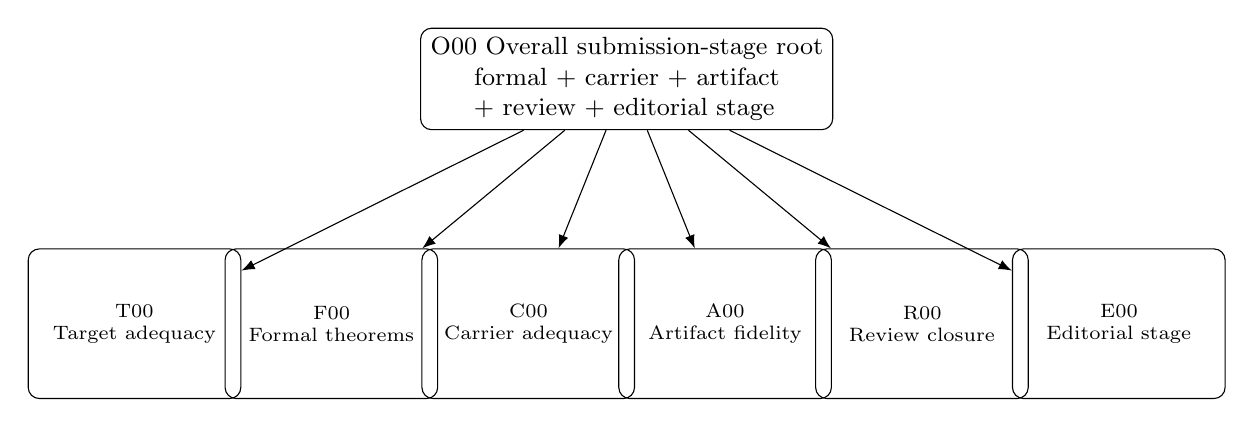
\begin{tikzpicture}[
  >=Latex,
  root/.style={draw,rounded corners,align=center,text width=50mm,minimum height=12mm,font=\small},
  fam/.style={draw,rounded corners,align=center,text width=24mm,minimum height=19mm,font=\scriptsize,inner sep=1.5mm},
  edge/.style={->,thin}
]
\node[root] (r) {O00 Overall submission-stage root\\formal + carrier + artifact + review + editorial stage};
\node[fam,below=15mm of r,xshift=-62.5mm] (t) {T00\\Target adequacy};
\node[fam,below=15mm of r,xshift=-37.5mm] (f) {F00\\Formal theorems};
\node[fam,below=15mm of r,xshift=-12.5mm] (c) {C00\\Carrier adequacy};
\node[fam,below=15mm of r,xshift=12.5mm] (a) {A00\\Artifact fidelity};
\node[fam,below=15mm of r,xshift=37.5mm] (rv) {R00\\Review closure};
\node[fam,below=15mm of r,xshift=62.5mm] (e) {E00\\Editorial stage};
\foreach \x in {t,f,c,a,rv,e} \draw[edge] (r)--(\x);
\end{tikzpicture}
\caption{Version-23 carrier-complete root.  A live recommendation-changing defect in any family prevents overall $\GCsub$.}
\label{fig:carrier-genome}
\end{figure}

The carrier family includes current journal scope, word and page limits, theorem centrality, theorem-level novelty, significance, related-work comparison, self-containment, notation and local orientation, and the final integrated recommendation.  The artifact family includes LaTeX/PDF identity, qpdf checks for both PDFs, rendered-page inspection, package hashes, Lean build and axiom audit, theorem-to-Lean correspondence, trace validation, and evidence provenance.  The review family requires a fresh independent trace, typed import of every recommendation-changing objection, node-specific Choice and execution records, and a second-order audit of the root certificate.

\begin{proposition}[Carrier-complete input traceability]\label{prop:instance}
Every load-bearing formal theorem, carrier invariant, artifact claim, review-validity condition, and submission-stage root condition is mapped to a node, a registered summary relation, or a typed omission witness in the seventy-one-node genome.
\end{proposition}

\paragraph{Expected versus actual status.}
Version 23 is drafted under the expected result
\[
  V_{\mathrm{expected}}=\ExpectedOverallGCA.
\]
At package construction time, however, the actual status is
\[
  V_{\mathrm{actual}}=\ActualOverallGCA,
\]
because no independent carrier-complete trace has yet passed the target-adequacy, qpdf, Lean, substantive-warrant, and root-aggregation gates.  The status include file is generated from the machine-readable execution-status record.  Claude Code is instructed to treat the expected result as adversarially untrusted, execute the frozen instance, and update the status only from the actual trace.  If the return is not $\GCsub$, the manuscript must be revised to reflect the actual result rather than preserving the assumption.

The package contains no author-issued carrier-complete root certificate.  It contains a non-executable template, schemas, proposal records, and scripts.  A valid independent result requires: a target-adequacy certificate; qpdf exit-zero certificates bound to the final PDF hashes; the actual Lean build certificate and theorem-coverage audit; a fresh conventional review whose recommendation-changing objections are imported as typed challenges; complete Choice and execution records; a substantive-warrant report; a second-order trace audit; and a root certificate integrating the journal recommendation.  Absence or failure of any required output leaves the status at $\NE$ or, after a valid bounded run, $\UB$.


\section{Countermodels and failure tests}

\begin{example}[Conventional review mislabeled as global]
A reviewer lists ordinary objections and predicts that a global traversal would reject the paper, but supplies no typed challenges, Choice records, executions, or root aggregation.  The output is $\NE$, not $\GI$.
\end{example}

\begin{example}[Unbounded elaboration demand]
A reviewer requests implementations of every parameterized state space, then semantics for each implementation language, then validators for those semantics, without identifying any variation capable of changing the fixed root verdict.  The requests do not become global challenges and the objects remain conditionally accepted.
\end{example}

\begin{example}[Trace laundering]
A syntactically populated trace repeats ``target complete'' and ``global action best'' at every node but supplies no node-specific projected outcomes or evidence.  The anti-laundering rule rejects the trace structurally.
\end{example}

\begin{example}[$\NE$ confused with $\UB$]
A model fails to produce a trace and reports undetermined within budget.  Because no traversal consumed a budget or reached a bounded stop state, the correct report is $\NE$.
\end{example}

\begin{example}[Indirect parent-mode transmission]
The successor input omits a field named parent mode but candidate generation reconstructs it from history and emits the same mode.  Mode-history erasure fails to commute with candidate generation, so noninterference is not established.
\end{example}

\begin{example}[Finite nonterminal deadlock]
A well-founded measure cannot descend infinitely, but a reachable nonterminal state has no validated successor.  Termination with a verdict does not follow; progress totality is missing.
\end{example}

\begin{example}[Leastness without proof]
Two incomparable inclusion-minimal operand graphs are target complete.  Calling either the unique least graph is false.  A policy-fixed selector can choose one without asserting uniqueness.
\end{example}

\begin{example}[Schema validation mistaken for warrant]
A validator confirms identifiers, hashes, budgets, and Choice arithmetic, but the cited mathematical counterexample is invalid.  $\TraceWF$ holds while $\TraceW$ fails.
\end{example}


\begin{example}[Target laundering]
A trace freezes a target that excludes novelty and significance, returns model-internal $\GC$, and reports major revision as a separate carrier verdict.  Two package states can share the frozen verdict while receiving different requested submission verdicts, so Theorem~\ref{thm:target-selection} identifies a residual pair.  The overall assessment is not executed for the requested target.
\end{example}

\begin{example}[Expected result used as evidence]
An author records $\GCsub$ as the expected audit result and allows that record to influence candidate fitness or root aggregation.  Execution-output separation fails because the anticipated conclusion has become a premise.  Version 23 freezes the expected result only as non-evidential metadata and begins with actual status $\NE$.
\end{example}

\begin{example}[Formal coherence plus major revision]
The formal family closes, but a fresh carrier review identifies an unresolved theorem-overstatement defect that changes the recommendation to major revision.  The carrier condition remains active, so the overall root cannot return $\GCsub$.  Choice may emit claim narrowing, manuscript revision, or bounded halt; it may not detach the recommendation and preserve $\GCsub$.
\end{example}

\begin{example}[qpdf tool unavailability]
The package requires a structural PDF warrant, but qpdf is unavailable in one environment.  Tool absence is not mathematical incoherence.  Before a hash-bound equivalent warrant exists, the artifact child remains active and overall $\GCsub$ is unavailable.  Claude Code may install qpdf or consume an externally generated certificate for the exact frozen PDF hashes.
\end{example}



\section{Relation to adjacent formal systems}

This section locates the results among information comparison, abstraction refinement, metareasoning, proof control, argumentation, and assurance cases.  The novelty claim concerns the integrated theorem family rather than the elementary kernel observation alone.

Blackwell comparison orders statistical experiments by their ability to support decision problems.  The target-relative residue construction is compatible with this decision-relative view: an observation is sufficient exactly when it preserves the distinctions needed by the fixed verdict.  The present factorization result is elementary relative to that tradition.  Its role here is to provide a representation-independent obstruction that is reused at three levels: native observation sufficiency, admissible-completion closure, and target-selection adequacy.

Abstract interpretation studies sound abstraction, fixpoint approximation, completeness, and refinement \cite{cousotcousot1977}.  Counterexample-guided abstraction refinement uses counterexamples to expose spurious behaviors and refine an abstraction \cite{clarke2000}.  A residual pair is more general than a spurious counterexample: it is any pair identified by an operative observation and separated by the selected target.  The universal splitting theorem says what every successful refinement must do without committing to one abstract domain.

Three-valued and generalized model checking retain an unknown result when a partial state space is insufficient \cite{brunsgodefroid1999,brunsgodefroid2000}.  The verdict $\UB$ is related but operationally richer: it records the bounded terminal state of a Choice-gated traversal together with the exact unresolved residue, conditions, and budget history.  $\NE$ is kept separate so that failure to execute the method cannot masquerade as a bounded semantic result.

Rational metareasoning and value-of-computation approaches compare computational actions according to their expected contribution to an objective.  The FMI Choice function belongs to this general family.  The specific result developed here is not the generic idea of choosing a computation.  It is the composition of total target-relative fitness comparison with target-relative residue, parent-mode information-flow erasure, conditional claim propagation, finite functional-genome history, and a trace-gated root verdict over heterogeneous native proof and carrier contexts.

Multi-strategy proof planning also uses meta-level control to select among proof methods.  The local/global distinction in this paper is not a fixed catalogue of proof tactics: it concerns the support required by the current target.  The strict separation theorems show why a recursive controller must be able to emit a local proof check from a global parent and a global bridge assessment from a local parent.

Proof-carrying code and certifying model checking attach checkable evidence to transmitted results \cite{necula1997,namjoshi2001}.  Foundational proof-certificate frameworks expose proof evidence through small trusted checker interfaces \cite{heathmiller2015}.  Choice and root certificates are control and composition certificates; they do not replace native mathematical proofs.  The Lean artifact certifies only the declarations it actually encodes, while qpdf certifies only the structural conditions detected by that tool.

Structured argumentation distinguishes claims, supports, attacks, and acceptability semantics \cite{dung1995,prakken2010}.  Assurance cases connect claims to evidence and have been integrated with formal proof artifacts \cite{foster2021}.  A functional genome adds typed execution contexts, candidate projection, target-relative mode selection, persistent history, conditional child interfaces, and a versioned transition semantics.  It is therefore an executable assessment state rather than only an argument diagram.

The integrated contribution is the following closure architecture: a requested target is tested for sufficiency; every recursive action is reselected by target-relative fitness; the terminal trace is interpreted over admissible completions; and the journal carrier is assessed inside the same root as the theorem package.  The carrier result is not allowed to compensate for a false theorem, but neither may a coherent theorem compensate for an unresolved recommendation-changing carrier defect.


\section{Discussion}

The global-coherence function is a configurable controller over typed native assessments, not a demand to implement every object that can be named.  Operand customization fixes a finite boundary; context customization fixes native semantics; the candidate grammar fixes the finite action space; and conditional acceptance preserves unresolved dependencies without converting them into unconditional warrant.  A request for more detail is globally active only when it identifies an admissible variation capable of changing the fixed root verdict.

Carrier completeness changes the stopping rule without making it unbounded.  Novelty, significance, scope, legibility, artifact fidelity, and the integrated recommendation are finite registered coordinates.  Each can remain conditionally accepted until challenged, but none may be silently discarded when it can change the submission verdict.  The submission-stage target stops before the future editorial decision while registering that decision as a successor-stage condition.

A prompt alone cannot guarantee execution by a large language model.  Version 23 externalizes the control state through schemas, a project-level \texttt{CLAUDE.md}, frozen hashes, check scripts, and a verdict output gate.  These controls still do not make a semantic review automatic.  The structural validator can reject missing actions, broken chains, unsupported verdict labels, absent carrier nodes, or a major-revision recommendation paired with $\GCsub$.  It cannot prove a mathematical theorem, establish novelty, or determine whether a challenge is genuinely recommendation changing.  Those judgments require node-specific substantive warrant and remain defeasible.

The expected $\GCsub$ result is deliberately placed outside the assessed evidence.  This lets the package be written toward a clear closure target without allowing that target to influence the audit.  The independent reviewer must be able to return $\GI$, $\UB$, or $\NE$, and the status-update script must rewrite the manuscript metadata accordingly.  The package is therefore a testable attempt to close, not a self-issued closure certificate.

The provisional Lean source is similarly non-load-bearing before compilation.  A clean build must record the toolchain, exact commands, source hashes, theorem inventory, warnings, and an axiom/placeholder audit.  The theorem-correspondence table distinguishes fully formalized, partially formalized, computationally checked, schema-represented, and unformalized results.  The qpdf certificate is likewise hash bound and limited to the exit status actually returned by \texttt{qpdf --check}; it is not a general proof of visual or semantic PDF correctness.

\section{Claude Code carrier-assessment protocol}

Claude Code begins in the package root, where the project-level \texttt{CLAUDE.md} is loaded as persistent project context.  The audit must not reuse an author verdict.  Its mandatory sequence is:
\begin{enumerate}
  \item verify the artifact manifest and frozen instance hashes;
  \item run the environment and author-preflight scripts;
  \item build the LaTeX sources and run qpdf checks against the resulting exact PDF hashes;
  \item debug and build the Lean package, audit declarations for placeholders and unintended axioms, and complete the theorem-correspondence and build-certificate records;
  \item verify target adequacy before considering any root verdict;
  \item perform a fresh conventional Studia Logica review of correctness, originality, significance, scope, legibility, and artifact fidelity;
  \item import every recommendation-changing criticism as a carrier-typed challenge with a concrete variation and a path to the overall root;
  \item for every reopened node, compare all seven registered actions, execute only the Choice-selected action, and update the genome, residue, conditions, history, and budgets;
  \item perform a second-order audit of the trace and substantive-warrant report; and
  \item issue a root certificate only if the trace passes structural validation and substantive review.
\end{enumerate}

For $\GCsub$, the root certificate must show that all formal and carrier conditions close, all mandatory artifact warrants are hash bound, no recommendation-changing challenge survives, and the integrated recommendation is accept or accept subject only to edits proven root invariant.  If the trace is not executed, the result is $\NE$.  If it executes to its bounded stop with active root residue, the result is $\UB$.  If a defeating contradiction or incurable carrier failure survives, the result is $\GI$.

The exact commands and required outputs are supplied in the read-first Claude Code instructions and the executable scripts in the package.  The status updater refuses to write $\GCsub$ unless the root certificate, qpdf certificate, Lean certificate, independent trace, substantive-warrant report, and validator transcript exist and agree on the frozen hashes.

\section{Conclusion}

Target-relative residue identifies when an observation erases a distinction required by a target.  Empty residue is equivalent to unique factorization through the observation image; the target-image observation is canonical in the refinement preorder; refinement is residue monotone; and every target-sufficient successor separates every residual pair.

Applied to assessment design, the same theorem prevents target substitution.  A frozen model-internal target can certify the requested overall submission target only when the requested carrier verdict factors through it.  Model-internal $\GC$ combined with a recommendation of major revision supplies a counterexample to that factorization.

The Choice-gated calculus fixes a target, finite operand graph, contexts, bridges, action grammar, projected-fitness policy, and budgets before execution.  All candidate actions are totally comparable for the same target.  Parent-mode history is erased before candidate generation and comparison, and progress plus well-founded decrease yields a bounded terminal verdict.  The sound-closure theorem then connects a warranted terminal trace to all admissible completions, while the separation and projection-margin theorems establish nontrivial control properties.

For Studia Logica, the overall root includes the formal theorem family, carrier adequacy, artifact fidelity, review-objection closure, and submission-stage editorial status.  A detachable carrier verdict is prohibited.  Version 23 is written toward the expected result $\ExpectedOverallGCA$, but the actual pre-audit status is $\ActualOverallGCA$.  Only the independent Claude Code trace may change the external execution-status record; the frozen manuscript remains the assessed input.  This makes the final assertion of global coherence an output of the carrier-complete assessment rather than an assumption used to generate it.

\section*{Audit-status record}
Expected carrier-complete submission-stage result: \ExpectedOverallGCA.  Actual frozen-package status at author construction: \ActualOverallGCA.  The expected result is non-evidential metadata.  The actual status must be regenerated from the independent trace and root certificate.

\section*{Declarations}

\paragraph{Competing interests.} The author declares no competing interests.

\paragraph{Data and code availability.} The LaTeX source, carrier-complete functional genome, configuration records, schemas, review instructions, validators, qpdf scripts, and provisional Lean source are supplied with the package.  The Lean source is not represented as a completed build certificate until it has compiled in the recorded environment and the completed certificate has been attached.

\paragraph{Use of generative AI.} OpenAI ChatGPT was used as a drafting and consistency-checking assistant.  The author remains responsible for every claim and artifact.  Claude Code is designated as the independent execution environment for the carrier-complete audit; its eventual outputs remain review evidence rather than authorial premises.



\begin{thebibliography}{12}
\bibitem{brunsgodefroid1999}
Glenn Bruns and Patrice Godefroid.
Model Checking Partial State Spaces with 3-Valued Temporal Logics.
In \emph{CAV 1999}, LNCS 1633, 274--287, 1999.

\bibitem{brunsgodefroid2000}
Glenn Bruns and Patrice Godefroid.
Generalized Model Checking: Reasoning about Partial State Spaces.
In \emph{CONCUR 2000}, LNCS 1877, 168--182, 2000.

\bibitem{clarke2000}
Edmund M. Clarke, Orna Grumberg, Somesh Jha, Yuan Lu, and Helmut Veith.
Counterexample-Guided Abstraction Refinement.
In \emph{CAV 2000}, LNCS 1855, 154--169, 2000.

\bibitem{cousotcousot1977}
Patrick Cousot and Radhia Cousot.
Abstract Interpretation: A Unified Lattice Model for Static Analysis of Programs by Construction or Approximation of Fixpoints.
In \emph{POPL 1977}, 238--252.

\bibitem{dung1995}
Phan Minh Dung.
On the Acceptability of Arguments and Its Fundamental Role in Nonmonotonic Reasoning, Logic Programming and $n$-Person Games.
\emph{Artificial Intelligence} 77.2 (1995), 321--357.

\bibitem{foster2021}
Simon Foster, Yakoub Nemouchi, Mario Gleirscher, Ran Wei, and Tim Kelly.
Integration of Formal Proof into Unified Assurance Cases with Isabelle/SACM.
\emph{Formal Aspects of Computing} 33 (2021), 855--884.

\bibitem{heathmiller2015}
Quentin Heath and Dale Miller.
A Framework for Proof Certificates in Finite State Exploration.
\emph{Electronic Proceedings in Theoretical Computer Science} 186 (2015), 11--26.

\bibitem{namjoshi2001}
Kedar S. Namjoshi.
Certifying Model Checkers.
In \emph{CAV 2001}, LNCS 2102, 2--13, 2001.

\bibitem{necula1997}
George C. Necula.
Proof-Carrying Code.
In \emph{POPL 1997}, 106--119.

\bibitem{prakken2010}
Henry Prakken.
An Abstract Framework for Argumentation with Structured Arguments.
\emph{Argument and Computation} 1.2 (2010), 93--124.
\end{thebibliography}

\end{document}
